%09.10.2024, lecture 1

\section{Lecture 1}\label{sec:1} % TODO

Few reminders:

\begin{theorem}[Markov inequality]
    \label{thm:markov}
    If $X \geq 0$ is a random variable, $a > 0$ and $\E[X] < \infty$, then
    \[
        \Pr[X > a] \leq \frac{\E[X]} {a}
    \]
\end{theorem}

\begin{theorem}[Chebyshev inequality]
    \label{thm:chebyshev}
    \[
        \Pr[|X - \E[X]| > a] \leq \frac{\Var[X]} {a^2}
    \]
\end{theorem}

\begin{definition}
    A \emph{randomized algorithm} $A$ is an algorithm that may use random bits and gives an answer.
    \[
        \Pr[A(x) \neq f(x)] \leq \frac 1 3.
    \]
    This class called $\BPP$.
    In real world application we use $\frac 1 n$.
    Mostly we will use $\frac 1 3$.

    We will measure time complexity for a worst case scenario.
    Another way is to measure time complexity in expectation over random bits for the worst input.
    This class called $\ZPP$.
\end{definition}

\begin{definition}
    Suppose an algorithm $A$, we say it has \emph{one-sided error} if:
    This class called $\RP$.
    \begin{itemize}
        \item For each $x \in f^{-1}(0)$ we have $A(x) = 0$ for any random bits.
        \item For each $x \in f^{-1}(1)$ we have $\Pr[A(x) = 0] < \frac 1 3$.
    \end{itemize}
\end{definition}

\begin{statement}
    Given algorithm with good expectation we can get a good algorithm with two-sided error.
    Simply by stopping algorithm after $10 \cdot E[\text{Time}]$ steps.
    And in the same manner we can output not a random value in scenario when the time is up, but output zero instead.
\end{statement}

\begin{algorithm}[Quick sort] \label{alg:quick_sort}
    Given an array $A$ of $n$ numbers.
    We choose at random some $x \in A$ and split $A$ into
    \begin{align*}
        A_L &= \{y \in A \mid y < x\} \\
        A_R &+ \{y \in A \mid y > x\}
    \end{align*}
    Thus, sort $A_L$ and $A_R$, then combine them.
    Total running time is $O(n \log n)$ in average.
\end{algorithm}
\begin{proof}
    Assume that we are a given sorted array.
    Let $X_{i, j}$ for $j > i$ to be defined:
    \begin{align*}
        X_{i, j} = \begin{cases} 1 \text{, if we compared } a_i \text{ with } a_j \\ 0 \text{ otherwise} \end{cases}
    \end{align*}
    Hence, $\Pr[X_{1, 2}] = 1$.
    In general:
    \[
      \Pr[X_{i, j}] = \frac 2 {j - i + 1}.
    \]
    It is, because at some point of our algorithm we will divide $i$ from $j$, there are $j - i + 1$ elements between them.
    Hence, the probability to compare them is to pick either $i$ or $j$.

    Summing up, we conclude that overall we compare
    \[
        \E \sum_{i = 1}^{n - 1} \sum_{j = i + 1}^n X_{i, j} = \sum_{i = 1}^{n - 1} \sum_{j = i + 1}^n \frac 2 {j - i + 1} = \sum_{i = 1}^{n - 1} \sum_{k = 1}^{n - i} \frac {2} {k + 1} \leq \sum_{i = 1}^{n - 1} O(\log n) \leq O(n \log n). \qedhere
    \]

\end{proof}

\begin{theorem}
    The median of an array can be found in $O(n)$ time in expectation.
\end{theorem}
\begin{proof}
    We can use idea of quick sort to find the median in time $O(n)$ in expectation.
\end{proof}
\begin{theorem}[Sampling algorithm]
    The median of an array can be found in $O(n)$ time iterating through the array twice with probability $n^{-\frac14}$.
\end{theorem}
\begin{proof}
    A brief overview of the algorithm.
    Array in our head would be already sorted.
    Let's select a bunch of random elements from an array.
    Then, we will pick two of them.
    And then conclude that a median is between them.
    The median between two favourite one with high probability and the size of elements between chosen one would be small enough.
    See \Cref{fig:d7e283af-ed41-46dc-8260-f52e8efd658d}.
\begin{figure}[H]
    \centering
    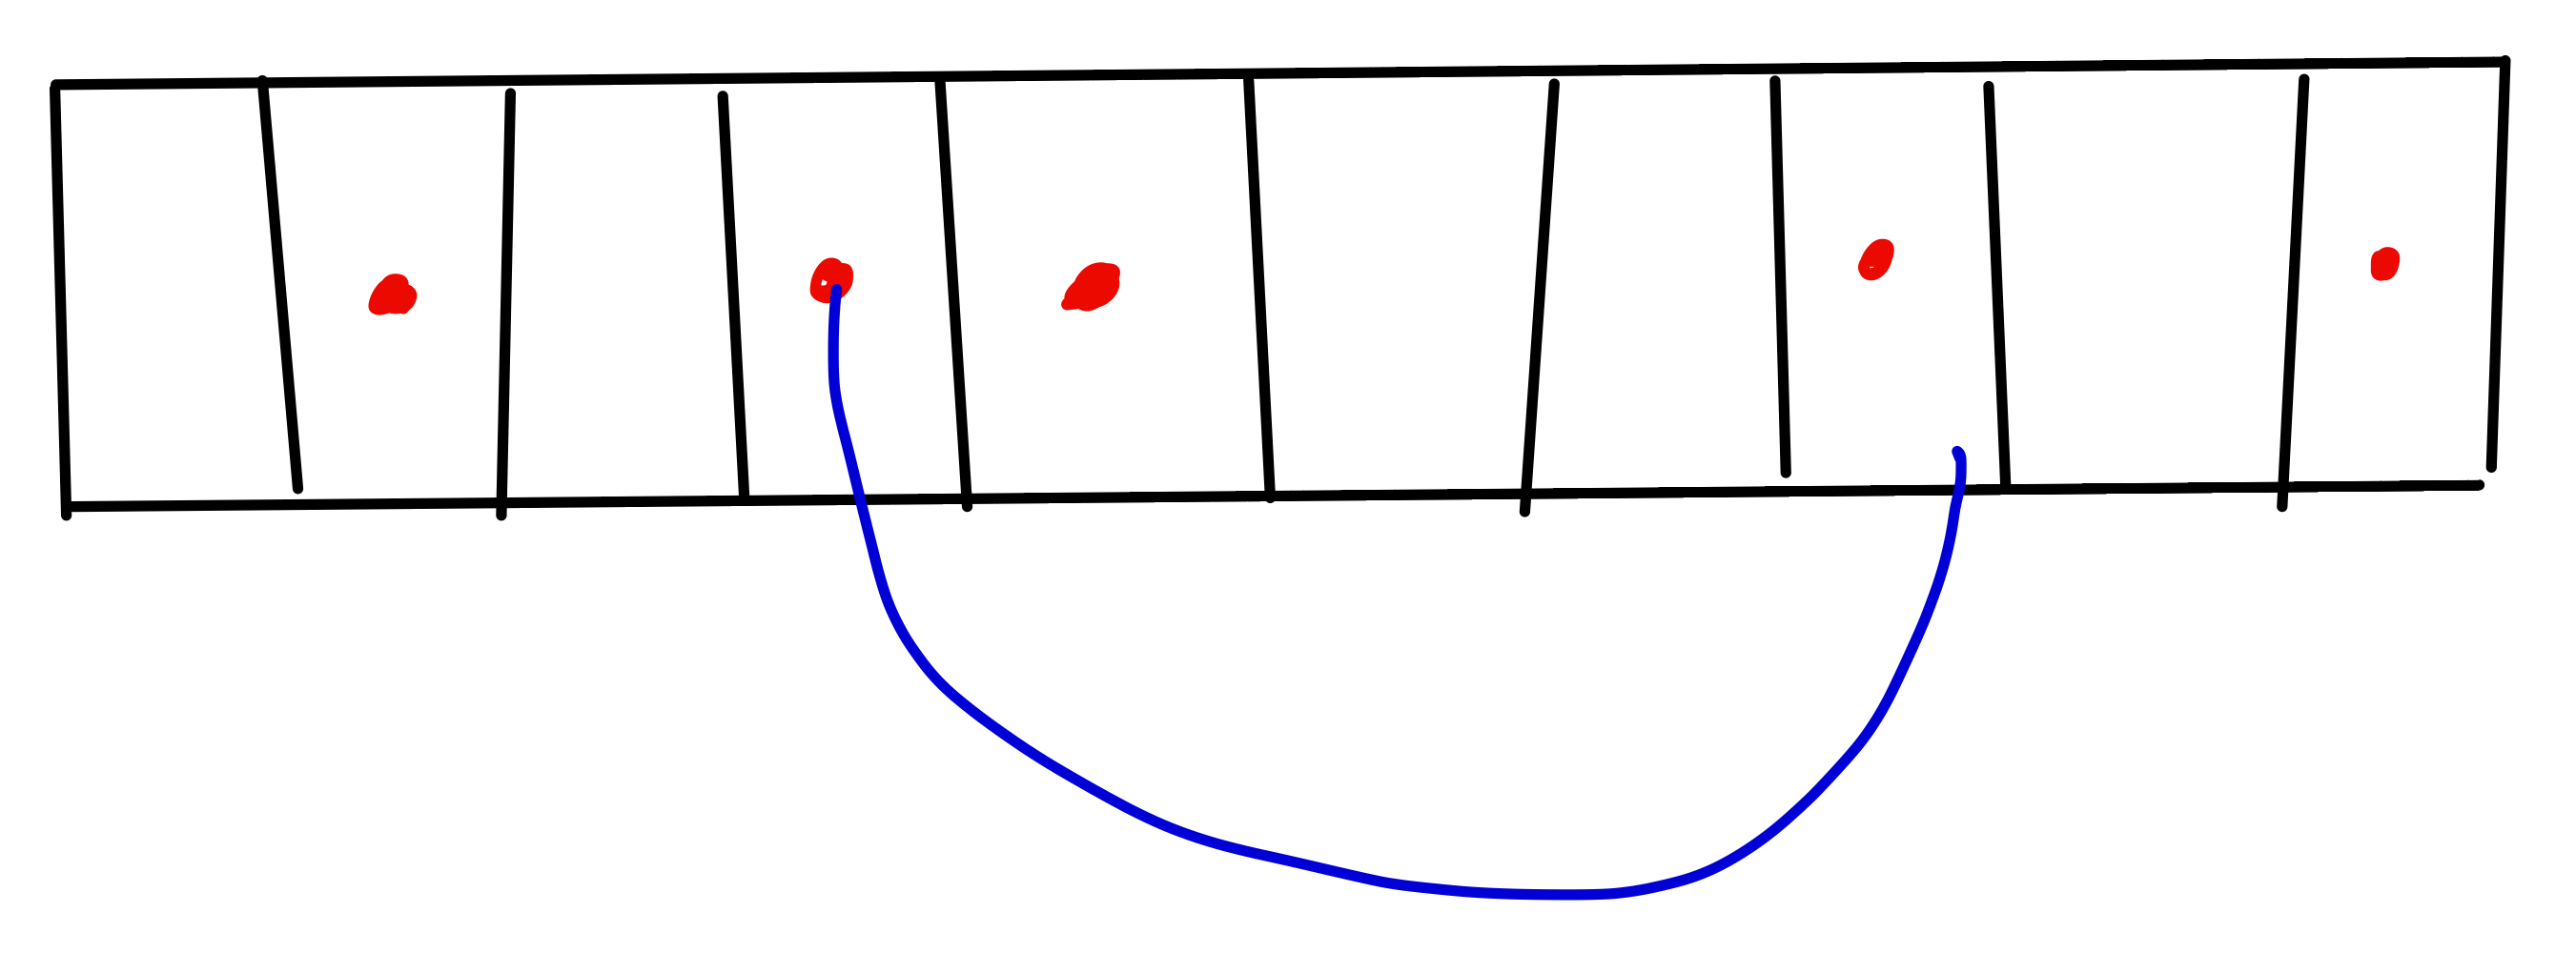
\includegraphics[width=0.4\textwidth]{figures/D7E283AF-ED41-46DC-8260-F52E8EFD658D}
    \caption{Idea of the median sampling algorithm}
    \label{fig:d7e283af-ed41-46dc-8260-f52e8efd658d}
\end{figure}
    Let's select $n^{\frac 3 4}$ points from the given array $A$ (all elements are distinct).
    Then, we will sort them.
    Chosen ones are $r_1, \ldots, r_{n^{\frac 3 4}}$ and $s_1, \ldots, s_{n^{\frac 3 4}}$ are the sorted ones.
    Let $x = s_{n^{\frac 3 4}/2 - \sqrt n}$ and $y = s_{n^{\frac 3 4}/2 + \sqrt n}$.
    Let $p(x)$ be a position of $x$ into the sorted array, i.e. $p(x) = \#\{y \in A \colon y \leq x\}$.
    Overall we have three chances to fail:
    \begin{enumerate}
        \item \label{itm:selecting_1} $p(x) > \frac n 2$
        \item \label{itm:selecting_2} $p(y) < \frac n 2$
        \item $p(y) - p(x) > 8 n^{\frac 3 4}$
    \end{enumerate}
    Assuming none of those happened, in one pass we can choose all $r_i$ and then obtain $s_i$ and find $x, y$.
    Hence, our median somewhere between $x, y$, those in the second pass we can find it.
    Let's estimate probabilities:
    Let $Y = [\# r_i \colon r_i > m]$, where $m$ is the median of $A$.
    Hence,
    \begin{align*}
        \Pr\left[p(x) > \frac n 2\right] = \Pr\left[Y > \frac{n^{\frac 3 4}}2 + \sqrt n\right] = \Pr\left[\sum_{i = 1} X_i > \underbrace{\frac{n^{\frac 3 4}}2}_{\E Y} + \sqrt n\right] \leq
    \end{align*} where $X_i = [r_i > m]$.
    Using \Cref{thm:chebyshev} we estimate this probability:
    \[
        \leq \Pr\left[ |\sum_{i = 1} X_i - \E[X_i]| > \sqrt n\right] \leq
    \]
    Estimating further:
    \[
        \Var[Y] = \sum_{i = 1}^n \Var[X_i] = \frac {n^{\frac 3 4}} 4.
    \]
    Hence,
    \[
        \leq \frac {n^{\frac 3 4}} {4 n} = \frac {1} {4 n^{\frac 1 4}}.
    \]

    Now, we will estimate the last one, that the size between $x, y$ is small enough.
    Intuitively, there are $\approx \sqrt n$ numbers $s_i$ between $x, y$ and the number of elements between each two $s_i$ is approximately $n^{\frac 1 4}$.
    Now, let's estimate it precisely.
    If $p(y) - p(x) > 8 n^{\frac 3 4}$, then one of the following is true:
    \begin{enumerate}
        \item $\frac n 2 - p(x) > 4 n^{\frac 3 4}$.
        \item $p(y) - \frac n 2 > 4 n^{\frac 3 4}$.
    \end{enumerate}
    Let's estimate the second one.
    Let $Y = \#\{r_i \colon m \leq r_i \leq a_{\frac n 2 + 4 n^{\frac 3 4}}\}$.
    Then, if $Y > 2 \sqrt n$, then $p(y) < \frac n 2 + 4 n^{\frac 3 4}$ (assuming that $p(x) \leq \frac n 2$).
    Because if $Y > 2 \sqrt n$ and $p(y) > \frac n 2 + 4n^{\frac 3 4}$, hence $p(x) > \frac n 2$.
    See \Cref{fig:de634714-a125-4fc2-8b73-33475238ecfc}.
    \begin{figure}[H]
        \centering
        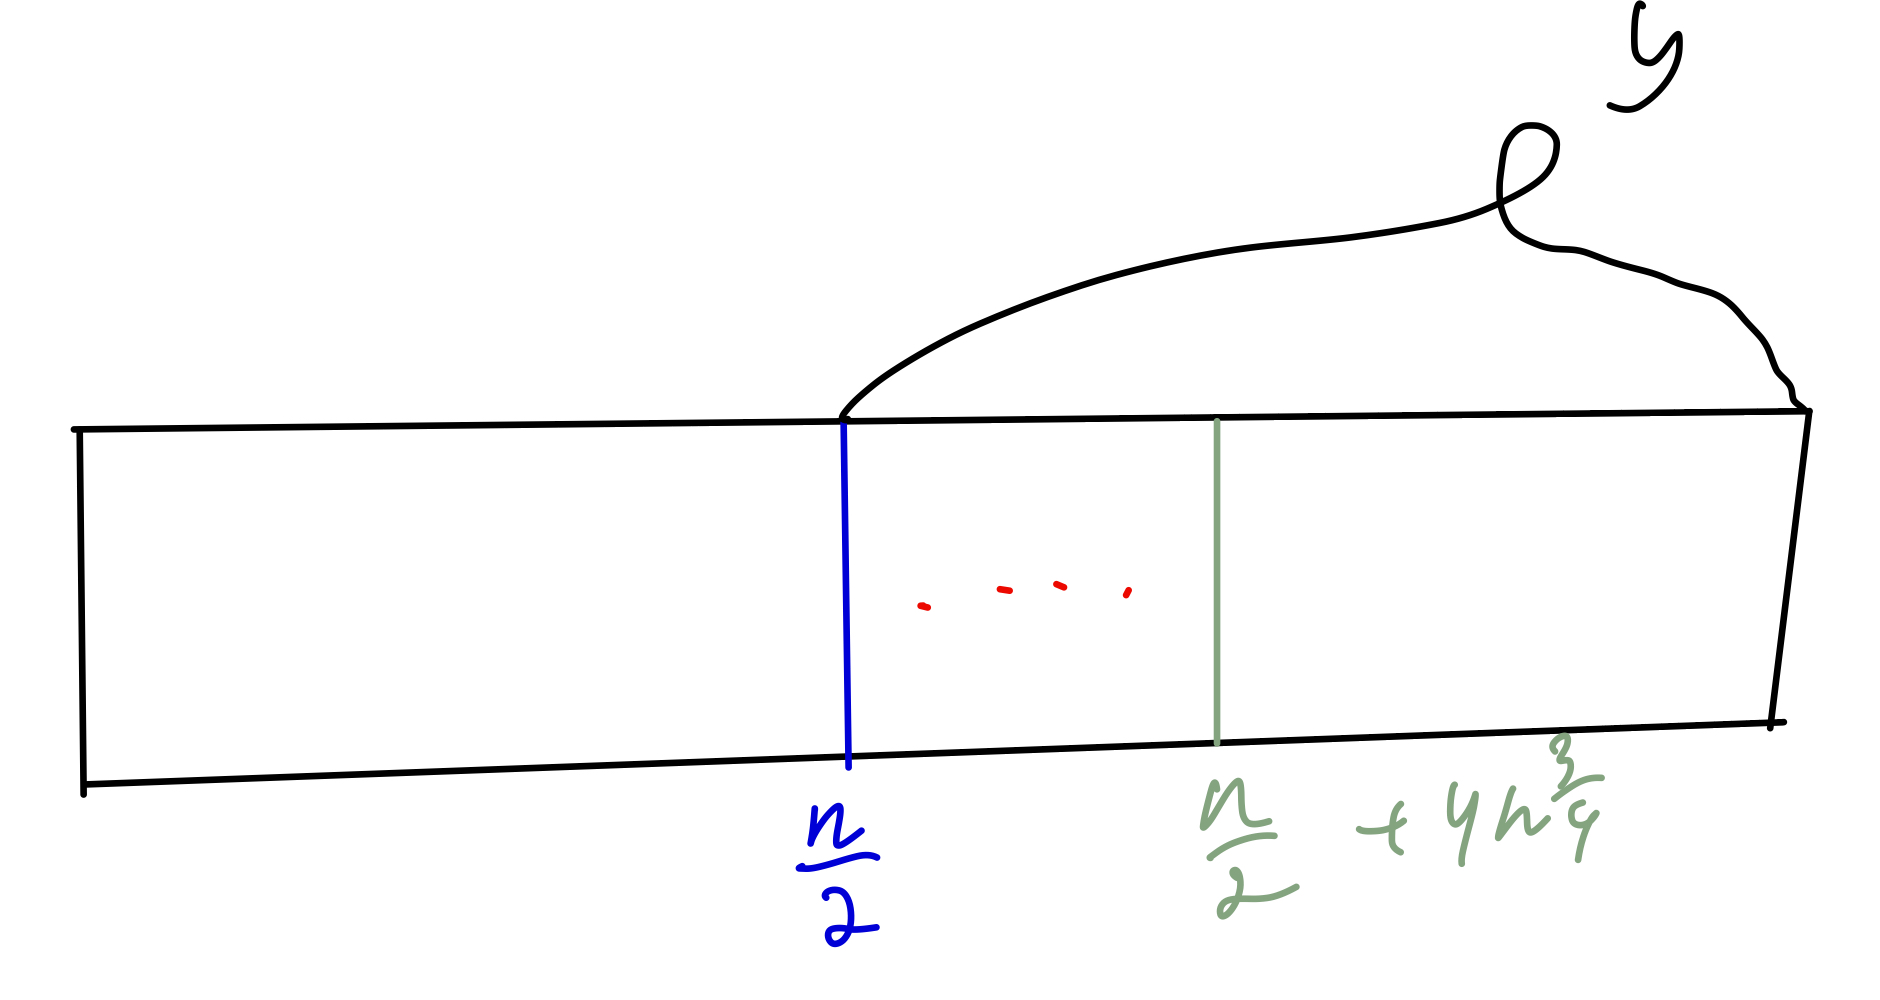
\includegraphics[width=0.5\textwidth]{figures/1052CAAC-783C-448C-AF25-B072B0C39DFB}
        \caption{Explanation of the last part of the proof.}
        \label{fig:de634714-a125-4fc2-8b73-33475238ecfc}
    \end{figure}

    Let $X_i = \left[m \leq r_i \leq a_{\frac n 2 + 4 n^{\frac 3 4}}\right]$.
    Hence,
    \[
        \E[Y] = \sum_{i = 1} \E[X_i] = n^{\frac 3 4} \cdot \frac{4 n^{\frac 3 4}}{n} = 4 \sqrt n.
    \]

    Now,
    \begin{align*}
        \Var[Y] &= \sum_{i = 1} \Var[X_i] = n^{\frac 3 4} \left(4 n^{-\frac 1 4} (1 - n^{-\frac 1 4})^2 + (1 - 4 n^{-\frac14}) (4 n^{-\frac14})^2\right) \approx \\
        &\approx n^{\frac 3 4} 4 n^{-\frac14} = 4 \sqrt n.
    \end{align*}

    Hence,
    \[
        \Pr\left[|Y - \E[Y]| > 2 \sqrt n\right] \leq \frac{4 \sqrt n}{4 n} = n^{-\frac 1 2}. \qedhere
    \]
\end{proof}

\begin{algorithm}[Cargo's]
    We have a graph and want to find a minimum cut.
    See \Cref{fig:1fd33d2b-a2e6-4129-b8b8-91ee68f24ac6}.
 \begin{figure}[H]
        \centering
        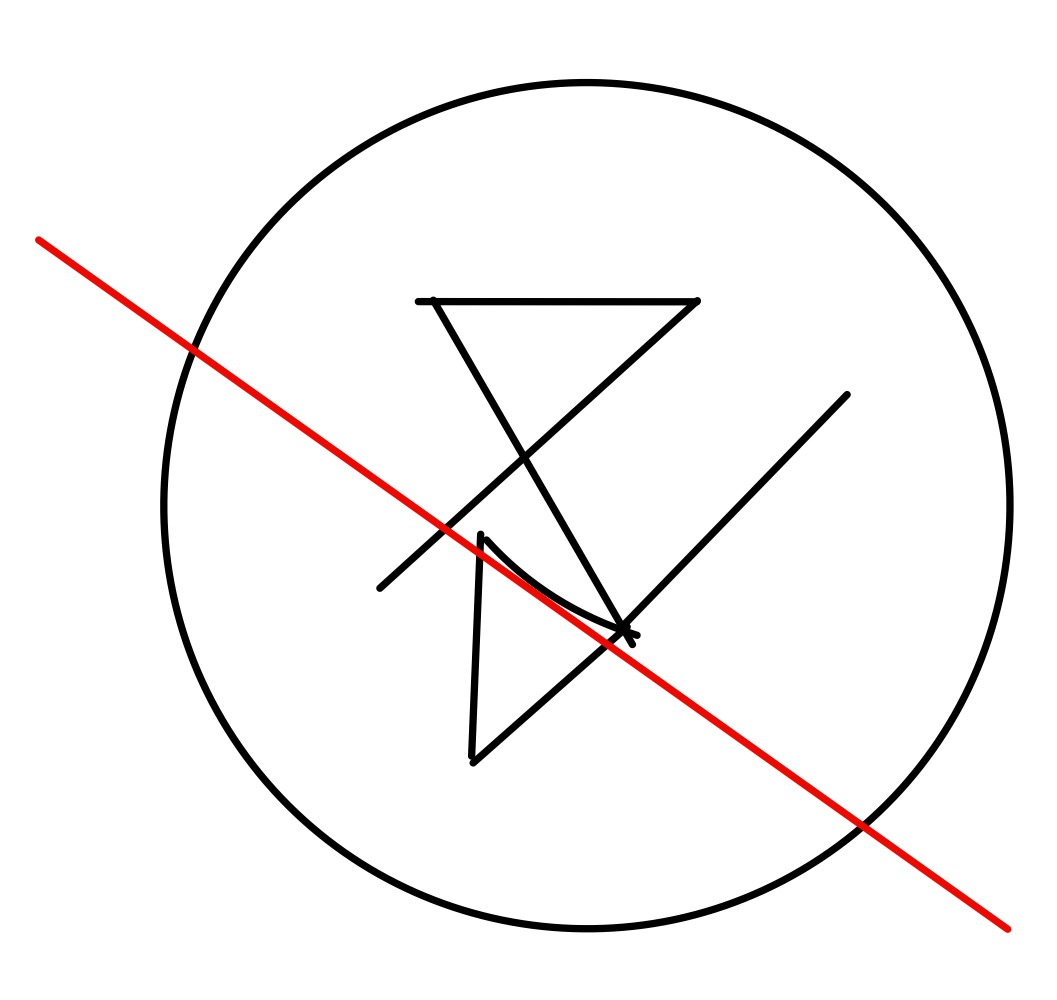
\includegraphics[width=0.35\textwidth]{figures/1FD33D2B-A2E6-4129-B8B8-91EE68F24AC6}
        \caption{Cut in a graph.}
        \label{fig:1fd33d2b-a2e6-4129-b8b8-91ee68f24ac6}
    \end{figure}
    Each time take random edge $(u, v)$ and merge $u$ and $v$ into a single vertex (with repeating edges).

    Running time is $O(n^2)$ and the probability of success is $\Omega(n^{-2})$.
    Hence, obtaining $O(n^4)$ algorithm with constant error probability.
\end{algorithm}
\begin{proof}
    The first edge $(u, v)$ that we have chosen edge is not from the minimal cut (which is fixed and we will call it $C$).

    Assume that the size of the minimal cut is $k$.
    Then $|E| \geq \frac {nk} 2$, since all degrees should be $\geq k$.
    Let $X_i$ be an event that we didn't pick an edge from $C$ on turn $i$ conditioned that we haven't picked any edges from $C$ on turn $1\ldots i - 1$.

    Hence,
    \[
        \Pr[X_1] \geq 1 - \frac {k} {\frac {nk} {2}} = \frac {n - 2} n.
    \]
    Hence, $\Pr[X_2] \geq \frac{n - 3}{n - 1}$, and so on.

    Therefore,
    \[
        \prod_{i = 1}^{n - 2} \Pr[X_i] = \frac{n - 2}{n} \cdot \frac{n - 3}{n - 1} \cdot \dots \cdot \frac 1 3 = \frac{2}{n (n - 1)}.
    \]
    We've just proved a funny theorem, it means that with probability $\frac{2}{n (n - 1)}$ we will obtain a minimal cut at the end, hence there is no more $\frac{n (n - 1)}{2}$ minimal cuts.
\end{proof}

\begin{algorithm}[Improved Cargo's] \label{alg:cargos_improved}
    As probability of success is decreasing and the amount of work is also decreasing, we will use branching.
    So, we can improve probability of success to $\Omega\left(\frac 1 {\log n}\right)$.
    And running time $O(n^2 \log n)$.
\end{algorithm}
\begin{proof}
    We will do our edges picking till the size of the graph became $\frac n {\sqrt 2}$.
    Hence, the probability would be
    \[
        \frac{n - 2}{n} \cdot \frac{n - 3}{n - 1} \cdot \dots \cdot \frac n {\sqrt 2} \approx \frac 1 2.
    \]

    We will do that and start branching on level $\frac n {\sqrt 2}$.
    In branching stage we do the same thing.
    So, the depth would be about $O(\log n)$.
    See \Cref{fig:39e45206-d894-4971-bfd2-a3a3a310c2b6}.
  \begin{figure}[H]
        \centering
        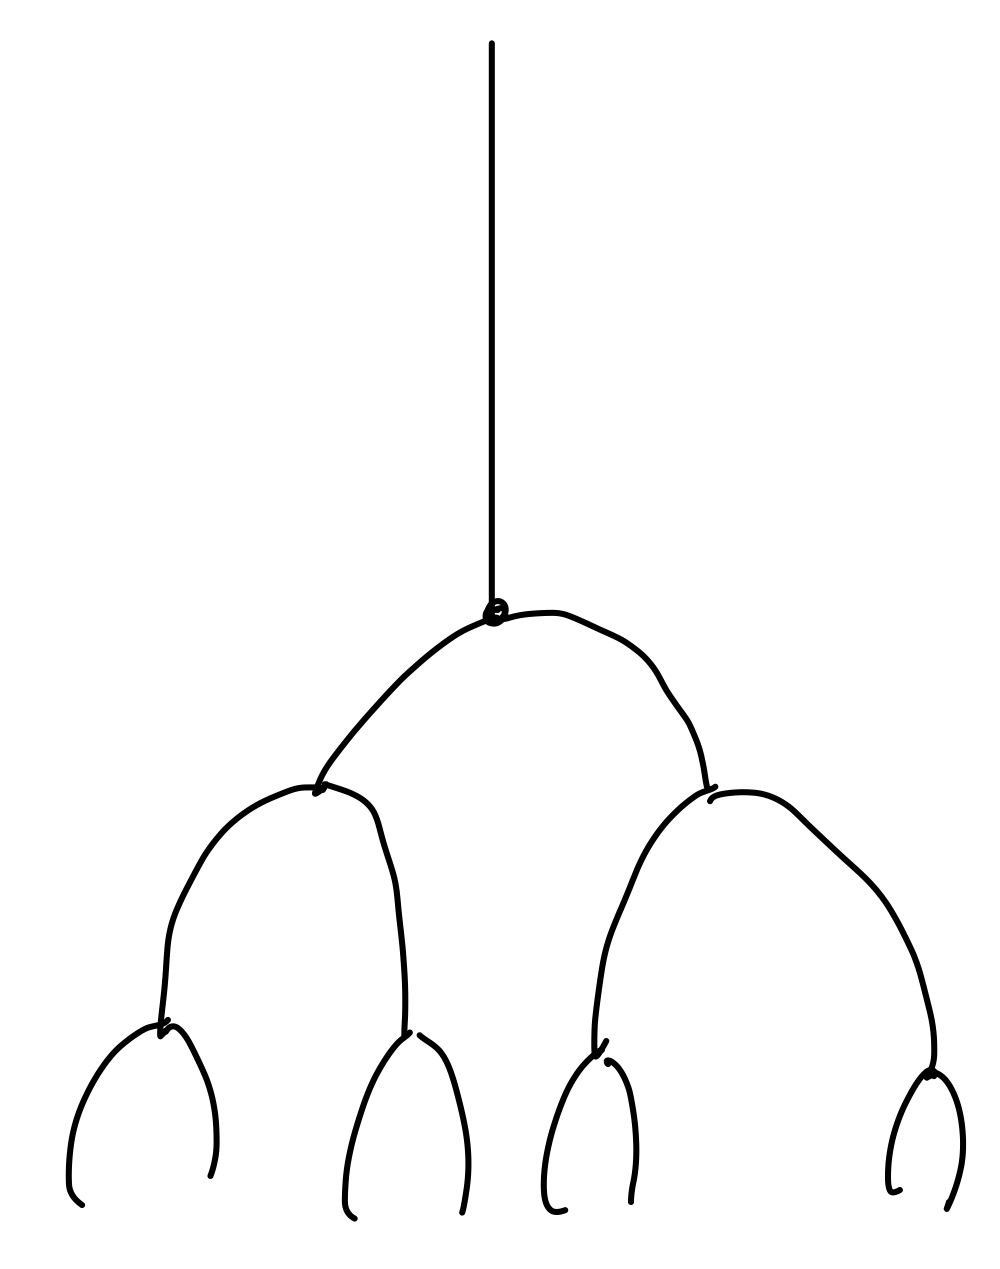
\includegraphics[width=0.25\textwidth]{figures/39E45206-D894-4971-BFD2-A3A3A310C2B6}
        \caption{Branching.}
        \label{fig:39e45206-d894-4971-bfd2-a3a3a310c2b6}
    \end{figure}

    Hence, if $p(n)$ is a probability of success on level $i$, hence:
    \[
        p(n) = \frac 1 2 - \left(1 - p\left(\frac n {\sqrt 2}\right)\right)^2.
    \]
    This implies that (by master theorem)
    \[
        p(n) = \Omega\left(\frac 1 {\log n}\right).
    \]

    And if the running time is $T(n)$, then:
    \[
        T(n) = O(n^2) + 2 T\left(\frac n {\sqrt 2}\right) = O(n^2 \log n). \qedhere
    \]
\end{proof}

\begin{algorithm}[Isolating cuts]
    Assume that in a graph some vertices are marked.
    We want to find a minimal cut that separates marked vertices from the rest.
    So one cut for each marked vertex (not at once).
\begin{figure}[H]
        \centering
        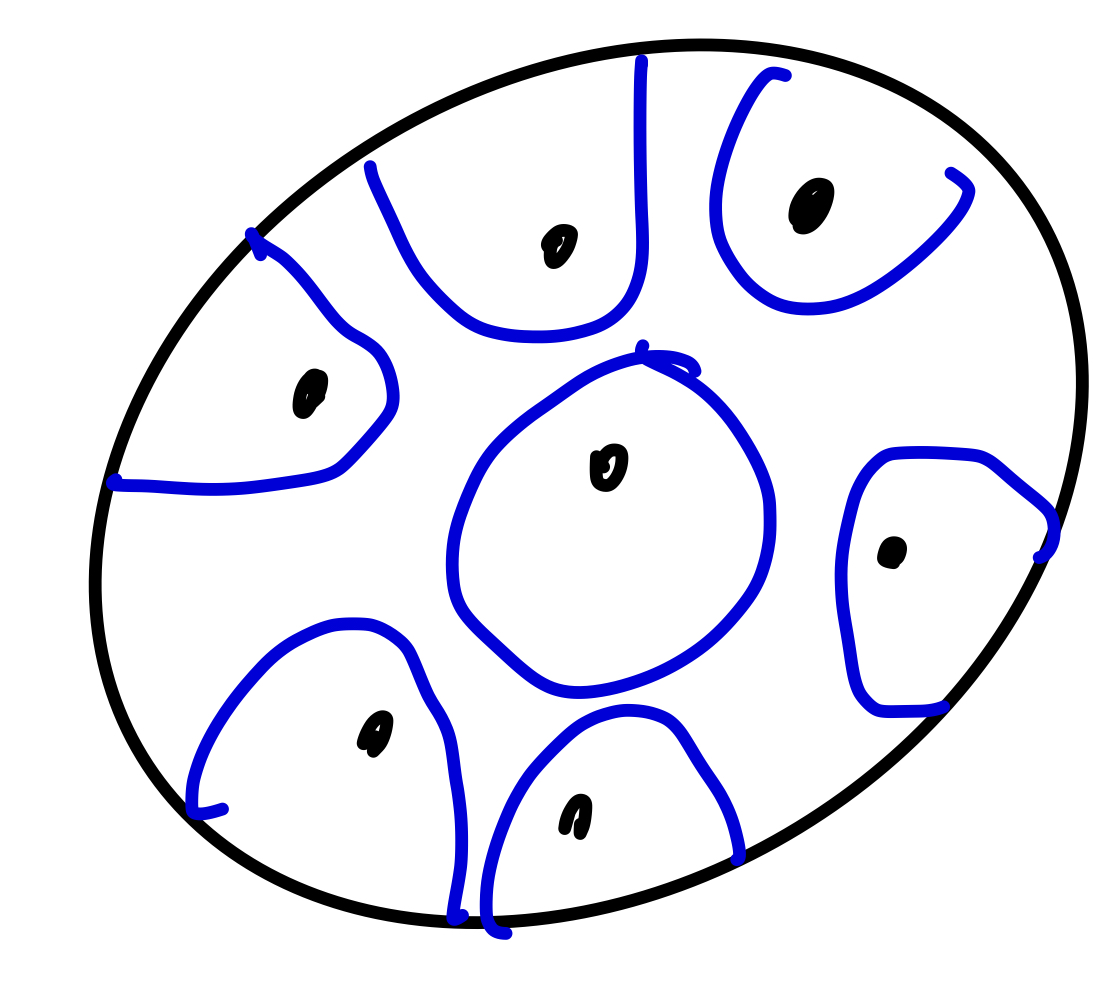
\includegraphics[width=0.4\textwidth]{figures/581ED485-1C5A-4F35-AF4B-8D1AB8E575EA}
        \caption{Isolated points.}
        \label{fig:581ed485-1c5a-4f35-af4b-8d1ab8e575ea}
    \end{figure}
\end{algorithm}
\begin{proof}
    If this set of size $k$, then we solve it in $k \cdot MC$.

\end{proof}